\subsection{Import PCAP Network Recording}
\label{sec:ui_import_pcap}

This task allows importing of ASTERIX data from a network recording stored as a PCAP file. \\

After selecting a PCAP file, the file is analyzed and an import dialog opens, showing a list of all network streams
found in the file. 

\begin{figure}[H]
    \center
      \hspace*{-0.5cm}
      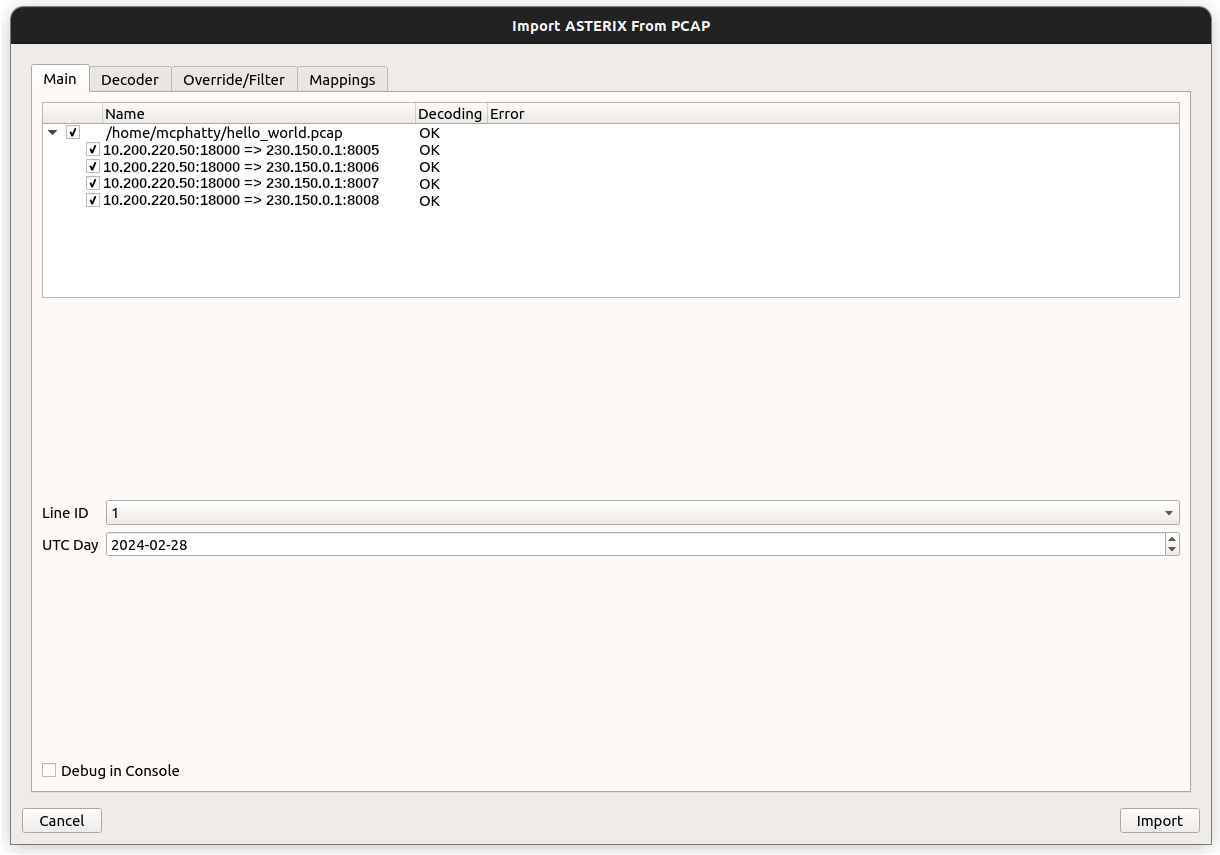
\includegraphics[width=17cm]{figures/asterix_import_pcap.png}
    \caption{Import ASTERIX from PCAP}
  \end{figure}

Such a network stream is always listed in the following format: \\

\textit{Source IP Address : Source Port => Destination IP Address : Destination Port} \\

For each network stream embedded byte data is collected and checked for valid ASTERIX data.
Network streams not containing valid ASTERIX data will be disabled and cannot be chosen for import.
A network stream containing valid ASTERIX data can be selected for import by using the data item's check box. \\

If one or more valid network streams are selected, the import can be carried out by clicking on the \textit{Import} button. \\

The other settings are similar to those in the ASTERIX file import, please refer to \nameref{sec:ui_import_asterix} for details. \\

Please \textbf{note} that in the case of a PCAP file the framing selection has no effect, since the data is always imported as raw/netto.

